
%%%%%
%%%%% DO NOT EDIT THIS FILE
%%%%%



\documentclass[12pt,a4paper,fleqn]{report}

%%% packages for mathematical typesetting
\usepackage{amsmath}
\usepackage{amssymb}
\usepackage{times}
\usepackage{bm}
%\usepackage{mathtools}
%\usepackage{nicefrac}
%\usepackage{latexsym}

%%% packages for including figures and subfigures
\usepackage{graphicx}
\usepackage[font=footnotesize,labelformat=empty]{subfig}

%%% package for nicer table layout
\usepackage{booktabs}

%%% package for color mangement
\usepackage[svgnames]{xcolor}

%%% package for page headings and footers
\usepackage{fancyhdr}

%%% package for hyperlinks
\usepackage{hyperref}
\hypersetup{%
  colorlinks=true,
  urlcolor=DarkGreen,
  citecolor=green,
  bookmarks=false}


\usepackage[noend]{algpseudocode}
\algrenewcommand\algorithmicdo{}
\algrenewcommand\algorithmicthen{}
\algrenewcommand{\algorithmiccomment}[1]{// #1}
\makeatletter
\newcommand{\StatexIndent}[1][3]{%
  \setlength\@tempdima{\algorithmicindent}%
  \Statex\hskip\dimexpr#1\@tempdima\relax}
\makeatother


\usepackage{fancyvrb} 
\usepackage{listings}
% Python style / environment for highlighting in "figures"
\lstdefinestyle{pythonstyle}{%
  language=Python,
  tabsize=4,
  backgroundcolor=\color{Gray!10},
  basicstyle=\ttfamily\scriptsize,
  stringstyle=\color{ForestGreen},
  keywordstyle=\color{BlueViolet},
  commentstyle=\itshape\color{DarkRed!90},
  identifierstyle=,
  emphstyle=\color{Blue},
  frame=lines,	
  showstringspaces=false,
  morekeywords={range, len, self, lambda, from, import, as, False, True, enumerate, map, list, set, float, int, min, max, with}
  fancyvrb=true,
}
\lstnewenvironment{python}[1][]{\lstset{style=pythonstyle,#1}}{}





\graphicspath{{./Figures/}, {./Images/}}



%%% text highlighting
\newcommand{\keyword}[1]{\emph{\texttt{\color{blue}#1}}}
\newcommand{\alert}[1]{\emph{\texttt{\color{red}#1}}}


%%% sets
\newcommand{\set}[1]{#1}

%%% vectors, matrices, and tensors
\renewcommand{\vec}[1]{\bm{#1}}
\newcommand{\mat}[1]{\bm{#1}}
\newcommand{\ten}[1]{\bm{\mathcal{#1}}}

%%% trace, rank, and diagonal
\newcommand{\tr}[1]{\operatorname{tr} \bigl [ #1 \bigr ]}
\newcommand{\TR}[1]{\operatorname{tr} \Bigl [ #1 \Bigr ]}
\newcommand{\rk}[1]{\operatorname{rk} \bigl [ #1 \bigr ]}
\newcommand{\RK}[1]{\operatorname{rk} \Bigl [ #1 \Bigr ]}
\newcommand{\diag}[1]{\operatorname{diag} \bigl [ #1 \bigr ]}
\newcommand{\DIAG}[1]{\operatorname{diag} \Bigl [ #1 \Bigr ]}

%%% inverse and transpose
\newcommand{\inv}[1]{#1^{-1}}
\newcommand{\trn}[1]{#1^\intercal}
\newcommand{\invtrn}[1]{#1^{-\intercal}}

%%% outer product
\newcommand{\opt}[2]{#1 \trn{#2}}

%%% inner products
\newcommand{\ipt}[2]{\trn{#1} #2}
\newcommand{\iptb}[2]{\left( \ipt{#1}{#2} \right)}
\newcommand{\ip}[2]{\langle #1, #2 \rangle}
\newcommand{\Ip}[2]{\bigl \langle #1, #2 \bigr \rangle}
\newcommand{\ipa}[2]{\langle #1, #2 \rangle}
\newcommand{\Ipa}[2]{\bigl \langle #1, #2 \bigr \rangle}
\newcommand{\dsq}[2]{\bigl \lVert #1 - #2 \bigr \rVert^2}
\newcommand{\nrm}[1]{\bigl \lVert #1 \bigr \rVert^2}
\newcommand{\sdsq}[2]{\lVert #1 - #2 \rVert^2}
\newcommand{\snrm}[1]{\lVert #1 \rVert^2}


\newcommand{\st}{\operatorname{s.\!t.}}
\newcommand{\amin}[1]{\operatorname*{argmin}_{#1}}
\newcommand{\amax}[1]{\operatorname*{argmax}_{#1}}

\newcommand{\submax}[1]{#1_{\text{max}}}

\newcommand{\ci}{\perp\!\!\!\perp}
\newcommand{\prob}[1]{p\bigl( #1 \bigr)}
\newcommand{\cprob}[2]{p\bigl( #1 \bigm| #2 \bigr)}

%%% horizontal and vertical dash
\newcommand{\hdash}{\operatorname{\,{}---{}\,}}
\renewcommand{\vdash}{\arrowvert}





\pagestyle{fancy}
\lhead{\emph{Image Processing (1)}}
\rhead{\emph{Winter Term 2021/22}}
\cfoot{}

\frenchspacing

\setlength{\parskip}{1ex plus0.5ex minus0.5ex}

\setlength{\headheight}{15pt}

\def\thesection{\arabic{section}.}
\setlength{\parindent}{0pt}

\renewcommand{\familydefault}{\sfdefault}





\begin{document}

\subsection*{exercise 1}
\textbf{warm up}
\vspace{1cm}

\subsection*{solutions due}
until \textbf{November 7, 2021} at \textbf{23:59} via \textbf{ecampus}
\vspace{1cm}

\vfill


\subsection*{students handing in this solution set}

\begin{tabular*}{\textwidth}{l@{\extracolsep{\fill}}lll}
  \toprule
  last name & first name & student ID & enrolled with \\
  \midrule
  \midrule
  %%%
  %%% enter data of 1st student here (i.e replace the following place holders)
  %%%
  Bach
  & Franziska
  & 123456
  & B-IT / RWTH Aachen
  \\
  %%%
  %%% enter data of 2nd student here (i.e replace the following place holders)
  %%%
  Wolfe
  & Frank
  & 654321
  & Uni Bonn
  \\
  %%%
  %%% if necessary, i.e. if there are further students in your team, add rows to this table
  %%%
  \bottomrule
\end{tabular*}
\newpage










%%%%%
%%%%% DO NOT EDIT THE FOLLOWING
%%%%%

\subsection*{general remarks}

As you know, your instructor is an avid  proponent of open science and education. Therefore, \textbf{MATLAB implementations will not be accepted} in this course.

The goal of this exercise is to get used to practical image processing in python / numpy / scipy. There are numerous Web resources related to python programming; numpy and scipy are mostly well documented and matplotlib, too, comes with numerous tutorials. Play with the code that is provided. The tasks below are rather simple; if you do not have any ideas for how to solve them, just look around for ideas as to how it can be done.

Also, \textbf{do NOT use additional third party libraries such as \texttt{OpenCV} or \texttt{scikit-image} for the coding tasks in this course!}

Why not? Because our goal in this course and its exercises is to learn about theory and practice of image processing on a reasonably foundational level. Regarding practical implementations of image processing algorithms, solutions in C or even assembler would constitute the most foundational level but likely be unreasonable. While working with python / numpy / scipy is still foundational enough, working with libraries such as \texttt{OpenCV} or \texttt{scikit-image} is definitely not. 

Think of it like this: if you train yourself to become a library monkey then what are you going to do when you are supposed to solve a problem for which there is no convenient library function available? How can you be sure that you really learned how to turn mathematics into computer code if all you ever do is stitching together other people's solutions to seemingly related problems?

\textbf{When handing solutions, always strive for excellence!} Your code and results will be checked and need to be convincing, reproducible, and comprehensible. If your solutions meet these criteria and you can demonstrate that they work in practice, it is a \emph{satisfactory} solution.

A \emph{very good} solution requires additional efforts especially w.r.t. to readability of your code. If your code is neither commented nor well structured, your solution is not good! The same holds for your discussion of your results: these should be concise and convincing and demonstrate that you understood what the respective task  was all about. Striving for very good solutions should always be your goal!
 


\newpage

\subsection*{practical advice}



The problem specifications you'll find below assume that you work with python / numpy / scipy. They also assume that you have imported 
\begin{python}
import imageio
import numpy as np
import scipy.ndimage as img
\end{python}



\vfill
To read- and write images from- and to disc, you may use these functions
\begin{python}[emph={imageRead,imageWrite}]
def imageRead(imgname, pilmode='L', arrtype=np.float):
    """
    read an image file into a numpy array

    imgname: str
        name of image file to be read 
    pilmode: str
        for luminance / intesity images use 'L'
        for RGB color images use 'RGB'
    arrtype: numpy dtype
        use np.float, np.uint8, ...
    """
    return imageio.imread(imgname, pilmode=pilmode).astype(arrtype)


def imageWrite(arrF, imgname, arrtype=np.uint8):
    """
    write a numpy array as an image file
    the file type is inferred from the suffix of parameter imgname, e.g. '.png'

    arrF: array_like
        array to be written
    imgname: str
        name of image file to be written
    arrtype: numpy dtype
        use np.uint8, ...
    """
    imageio.imwrite(imgname, arrF.astype(arrtype))
\end{python}



\vfill
To display an intensity image on your screen, you could use the following
\begin{python}
import matplotlib.pyplot as plt

arrF = imageRead('portrait.png')
plt.imshow(arrF / 255, cmap='gray')
plt.show()
\end{python}



To display an (RGB) color image on screen, you might use
\begin{python}
import matplotlib.pyplot as plt

arrF = imageRead('../exercise1/Data/asterixRGB.png', pilmode='RGB')
plt.imshow(arrF / 255)
plt.show()
\end{python}




\subsection*{task 1.1 \\[1ex] the emboss effect}

In the \texttt{Data} folder for this exercise, you will find the intensity image
\begin{quote}
    \texttt{portrait.png}
\end{quote}
Read it into a numpy array \texttt{arrF} and print the shape of this array to determine its number of rows and columns.
\color{blue} \\[1ex]
%%%%%
%%%%%
%%%%% enter your result here
%%%%%
%%%%%
enter your result here \ldots
%%%%%
%%%%%
%%%%%
%%%%%
%%%%%
\color{black}

In the lecture, we discussed the idea of ``embossing'' an image such that the resulting image resembles a copper engraving. In fact, we discussed 4 different methods to accomplish this, namely
\begin{python}[emph={embossV1,embossV2,embossV3,embossV4}]
def embossV1(arrF):
    M, N = arrF.shape
    arrG = np.zeros((M,N))

    for i in range(1,M-1):
        for j in range(1,N-1):
            arrG[i,j] = 128 + arrF[i+1,j+1] - arrF[i-1,j-1]
            arrG[i,j] = np.maximum(0, np.minimum(255, arrG[i,j]))

    return arrG


def embossV2(arrF):
    M, N = arrF.shape
    arrG = np.zeros((M,N))
    
    arrG[1:M-1,1:N-1] = 128 + arrF[2:,2:] - arrF[:-2,:-2]
    arrG = np.maximum(0, np.minimum(255, arrG))

    return arrG


def embossV3(arrF):
    mask = np.array([[-1, 0,  0],
                     [ 0, 0,  0],
                     [ 0, 0, +1]])

    arrG = 128 + img.correlate(arrF, mask, mode='reflect')
    arrG = np.maximum(0, np.minimum(255, arrG))

    return arrG
    
  
def embossV4(arrF):
    arrG = 128 + arrF[2:,2:] - arrF[:-2,:-2]
    arrG[arrG<  0] =   0
    arrG[arrG>255] = 255

    return arrG
\end{python}

\newpage

Apply each of the above methods to \texttt{arrF} to produce a corresponding array \texttt{arrG} and write each of your results as a PNG image.

Does the result you obtain from \keyword{embossV4} differ from the results produced by the other methods? It should! Discuss the difference!
\color{blue} \\[1ex]
%%%%%
%%%%%
%%%%% enter your discussion here
%%%%%
%%%%%
enter your discussion here \ldots
%%%%%
%%%%%
%%%%%
%%%%%
%%%%%
\color{black}



\subsection*{task 1.2 \\[1ex] timing the emboss effect}

In the lecture, we also performed experiments to determine the minimum average runtime of our different methods for the \emph{emboss} effect. In this task you are supposed to conduct these experiments on your own machines.

Assuming that you have read an input intensity image into an array \texttt{arrF}, you may use the following code snippets for this purpose
\begin{python}
import timeit, functools


mtds = [embossV1, embossV2, embossV3, embossV4]

nRep =   3
nRun = 100
    
for mtd in mtds:
	ts = timeit.Timer(functools.partial(mtd, arrF)).repeat(nRep, nRun)
	print (min(ts) / nRun)
\end{python}



\begin{description}
\item[task 1.2(a):] In the \texttt{Data} folder, you will find the intensity image
\begin{quote}
    \texttt{portrait.png}
\end{quote}
Read it into an array \texttt{arrF}, print its shape, and run the above timing script.
\color{blue} \\[1ex]
%%%%%
%%%%%
%%%%% enter your result here
%%%%%
%%%%%
V1: 0.44967310061001625 \\
V2: 0.0007028839599661297 \\
V3: 0.0012256227100078832 \\
V4: 0.00038784879998274844 \\
%%%%%
%%%%%
%%%%%
%%%%%
%%%%%
\color{black}

\item[task 1.2(b):] In the \texttt{Data} folder, you will find the intensity image
\begin{quote}
    \texttt{asterix.png}
\end{quote}
Read it into an array \texttt{arrF}, print its shape, and run the above timing script.
\color{blue} \\[1ex]
%%%%%
%%%%%
%%%%% enter your result here
%%%%%
%%%%%
V1: 2.5130979724999998 \\
V2: 0.011546289530015201 \\
V3: 0.011558454990008613 \\
V4: 0.005792928150003718 \\
%%%%%
%%%%%
%%%%%
%%%%%
%%%%%
\color{black}

\newpage
\item[task 1.2(c):] Discuss your results. What do your experiments reveal? Is there any noteworthy difference between the runtimes for the two images? If so, what is the difference? What causes this difference? What does this tell you about image processing in general?
\color{blue} \\[1ex]
%%%%%
%%%%%
%%%%% enter your discussion here
%%%%%
%%%%%
The functions called on the second image take about 5.5 times longer, since the image has that much more pixels. The most noteworthy difference is between the first method and the others. The first takes far longer because it uses a python loop to iterate over all pixels, which are very slow compared to more low level programming languages. Meanwhile, numpy and scipy functions, like subtracting two arrays in methods 2 and 4, or the correlate function in 3, are implemented in C, where large loops are much faster.
%%%%%
%%%%%
%%%%%
%%%%%
%%%%%
\color{black}
\end{description}





\subsection*{task 1.3 \\[1ex] working with RGB color images}

In the \texttt{Data} folder, you will find the color image
\begin{quote}
    \texttt{asterixRGB.png}
\end{quote}
Read it into an array \texttt{arrF} using 
\begin{python}
arrF = imageRead('asterixRGB.png', pilmode='RGB')
\end{python}

Print the shape parameters of \texttt{arrF} and run the following snippet
\begin{python}
arrG = np.copy(arrF)
arrG[:,:,0] = 0
\end{python}

Write the resulting array \texttt{arrG} as a PNG file and enter it here
%%%%%
%%%%%
%%%%% enter your image here, i.e. replace "placeholder.pdf" by the name of the image file you created
%%%%%
%%%%%
\begin{center}
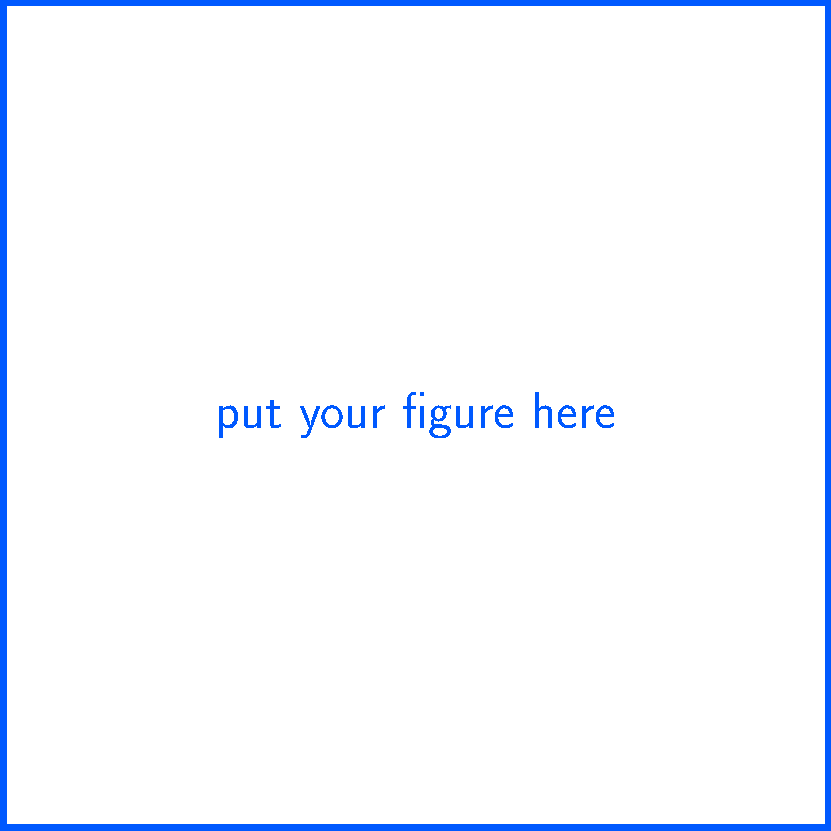
\includegraphics[width=0.5\textwidth]{placeholder.pdf} 
\end{center}
%%%%%
%%%%%
%%%%%
%%%%%
%%%%%





\subsection*{task 1.4 \\[1ex] getting used to slicing (part 1)}

Read image \texttt{asterix.png} into an array \texttt{arrF} and image \texttt{portrait.png} into an array \texttt{arrG}.

Now, create a copy \texttt{arrH} of \texttt{arrF} and then ---without using \keyword{for} loops--- paste \texttt{arrG} into \texttt{arrH} such that the upper left corner of \texttt{arrG} is at array coordinate $[i,j] = [100, 200]$ in \texttt{arrH}. Write your result as a PNG image.

To illustrate how this image should look like, here is the result you would obtain from using $[i,j] = [10, 10]$
%%%%%
%%%%%
%%%%% enter your result here, i.e. replace "t1-4.png" by the name of your resulting image file
%%%%%
%%%%%
\begin{center}
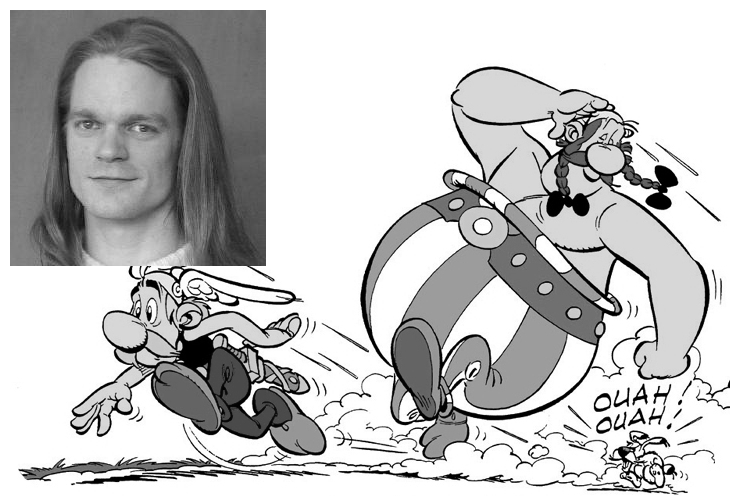
\includegraphics[width=0.5\textwidth]{t1-4.png} 
\end{center}
%%%%%
%%%%%
%%%%%
%%%%%
%%%%%
Simply replace the above image with the image you just created.








\subsection*{task 1.5 \\[1ex] getting used to slicing (part 2)}

Read image \texttt{portrait.png} into an array \texttt{arrF}. Then ---without using \keyword{for} loops--- set all the intensities of the pixels in in every $16$th column and every $16$th row of \texttt{arrF} to $0$. Write your result as a PNG image.

To illustrate how this image should look like, here is the result you would obtain from working with every $8$th row and column and setting intensities to $255$.
%%%%%
%%%%%
%%%%% enter your result here, i.e. replace "t1-5.png" by the name of your resulting image file
%%%%%
%%%%%
\begin{center}
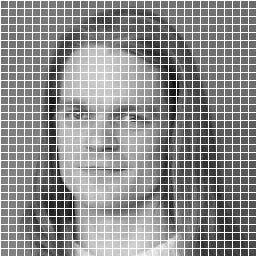
\includegraphics[width=0.5\textwidth]{t1-5.png} 
\end{center}
%%%%%
%%%%%
%%%%%
%%%%%
%%%%%
Simply replace the above image with the image you just created.








\subsection*{task 1.6 \\[1ex] getting used to meshgrids (part 1)}

Read image \texttt{portrait.png} into an array \texttt{arrF}. Then ---without using \keyword{for} loops--- set the intensities of all its pixels situated within an ellipse of width $2 \cdot 50$ and height $2 \cdot 85$ which is centered at array coordinates $\bigl[ c_i, c_j \bigr] = \bigl[ 128, 110 \bigr]$ to $255$. Write your result as a PNG image. \\[1ex]
%%%%%
%%%%%
%%%%% enter your code into the following environment
%%%%%
%%%%%
\begin{python}
# paste your code here

\end{python}
%%%%%
%%%%%
%%%%%
%%%%%
%%%%%



\vspace{1cm}
To illustrate how your resulting image should look like, here is the result you would obtain from working with width $2 \cdot 100$, height $2 \cdot 50$ and center point $\bigl[ 128, 128 \bigr]$
%%%%%
%%%%%
%%%%% enter your result here, i.e. replace "t1-6.png" by the name of your resulting image file
%%%%%
%%%%%
\begin{center}
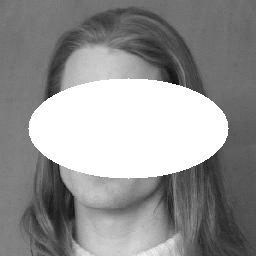
\includegraphics[width=0.5\textwidth]{t1-6.png} 
\end{center}
%%%%%
%%%%%
%%%%%
%%%%%
%%%%%
Simply replace the above image with the image you just created.








\subsection*{task 1.7 \\[1ex] getting used to meshgrids (part 2)}

Read image \texttt{portrait.png} into an array \texttt{arrF}. Then ---without using \keyword{for} loops--- create an image array \texttt{arrG} whose content looks like shown below
\begin{figure}[h!]
\begin{center}
\subfloat[\texttt{arrF}]{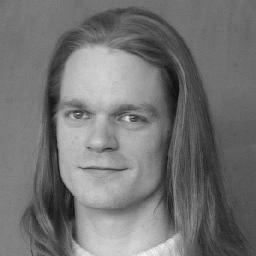
\includegraphics[width=0.45\textwidth]{portrait.png}} \hfill
\subfloat[\texttt{arrG}]{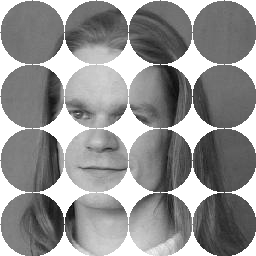
\includegraphics[width=0.45\textwidth]{t1-7.png}}
\end{center}
\end{figure}

\textbf{Note:} the circles in the above figure have a radius of $r = 32$ pixels. Implement your code such that it produces circles of radius $r \in \{ 16, 64 \}$ pixels. \\[1ex]
%%%%%
%%%%%
%%%%% enter your code into the following environment
%%%%%
%%%%%
\begin{python}
# paste your code here

\end{python}
%%%%%
%%%%%
%%%%%
%%%%%
%%%%%



\newpage
Perform runtime measurements for your code and paste your result here. (When implemented ``properly'', your solution should be able to process  \texttt{portrait.png} in only $O(10^{-5})$ seconds \ldots)
\color{blue} \\[1ex]
%%%%%
%%%%%
%%%%% enter your result here
%%%%%
%%%%%
enter your result here \ldots
%%%%%
%%%%%
%%%%%
%%%%%
%%%%%
\color{black}



\vspace{4cm}
Finally, enter your resulting images (for $r \in \{ 16, 64 \}$) here
%%%%%
%%%%%
%%%%% enter your result here, i.e. replace "placeholder.pdf" by the names of the image files you created
%%%%%
%%%%%
\begin{center}
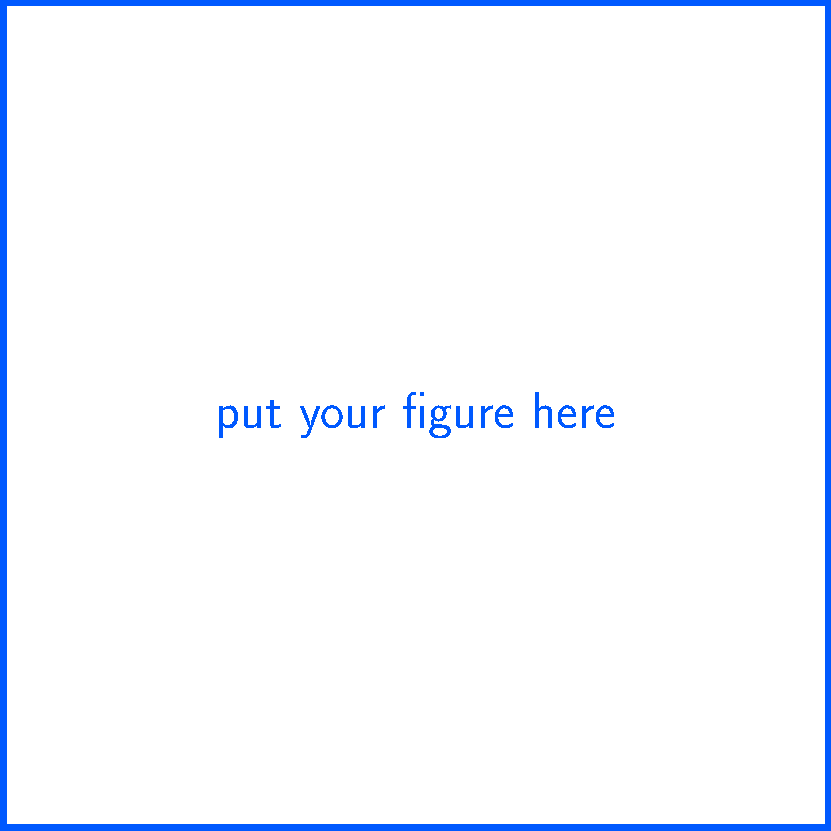
\includegraphics[width=0.45\textwidth]{placeholder.pdf} \hfill
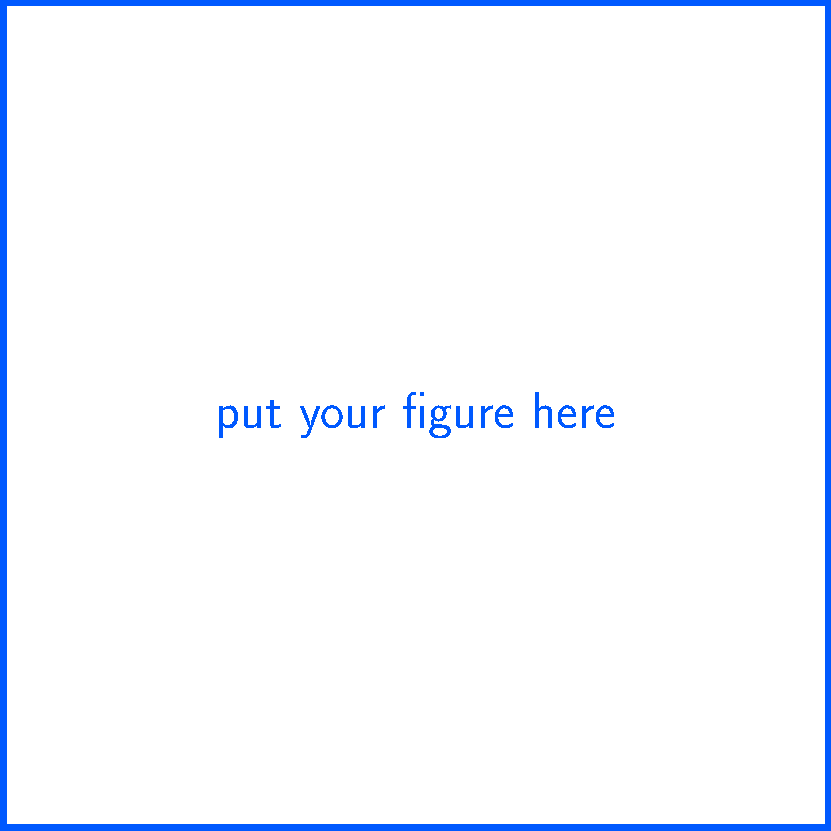
\includegraphics[width=0.45\textwidth]{placeholder.pdf} 
\end{center}
%%%%%
%%%%%
%%%%%
%%%%%
%%%%%








\subsection*{task 1.8 \\[1ex] getting used to meshgrids (part 3)}

Again ---without using \keyword{for} loops--- create an image of size $M \times N$ where $M = N = 256$ that displays the following function
\begin{equation*}
f \bigl[ x, y \bigr] = \frac{1}{2} \Bigl( \sin \bigl( 2\,\pi\,\nu \, \tfrac{x}{N-1} + \tfrac{\pi}{2} \, (N-1)\bigr) + 1 \Bigr) \cdot 255
\end{equation*}

For instance, when choosing the free parameter $\nu = 5$, your image should look like this
\begin{center}

\includegraphics[width=0.35\textwidth]{t1-8.png} 
\end{center}

\vspace{1cm}
Create such images for $\nu \in \{ 1, 2, 3, 9 \}$ and paste them here
%%%%%
%%%%%
%%%%% enter your results here, i.e. replace "placeholder.pdf" by the names of the image files you created
%%%%%
%%%%%
\begin{center}
\includegraphics[width=0.24\textwidth]{t8-1.png} \hfill
\includegraphics[width=0.24\textwidth]{t8-2.png} \hfill
\includegraphics[width=0.24\textwidth]{t8-3.png} \hfill
\includegraphics[width=0.24\textwidth]{t8-5.png} 
\end{center}
%%%%%
%%%%%
%%%%%
%%%%%
%%%%%



\newpage
Also, paste your code here \\[1ex]
%%%%%
%%%%%
%%%%% enter your code into the following environment
%%%%%
%%%%%
\begin{python}
def f(nu, M=256, N=256):
    xx, yy = np.meshgrid(range(M), range(N), indexing='xy')
    return .5 * (np.sin(2 * np.pi * nu * xx / (N - 1) + .5 * np.pi * (N - 1)) + 1) * 255

\end{python}
%%%%%
%%%%%
%%%%%
%%%%%
%%%%%







\subsection*{task 1.9 \\[1ex] getting used to meshgrids (part 9)}

Again ---without using \keyword{for} loops--- create an image of size $M \times N$ where $M = N = 256$ that displays the following function
\begin{equation*}
f \bigl[ x, y \bigr] = \frac{1}{2} \Bigl( e^{-\frac{4\,y}{M}}\sin \bigl( 2\,\pi\,\nu \, \tfrac{y}{M-1} + \tfrac{\pi}{2} \, (M-1)\bigr) + 1 \Bigr) \cdot 255
\end{equation*}

For instance, when choosing the free parameter $\nu = 7$, your image should look like this
\begin{center}

\includegraphics[width=0.35\textwidth]{t1-9.png} 
\end{center}

\vspace{1cm}
Create such images for $\nu \in \{ 5, 9, 11, 13 \}$ and paste them here
%%%%%
%%%%%
%%%%% enter your results here, i.e. replace "placeholder.pdf" by the names of the image files you created
%%%%%
%%%%%
\begin{center}
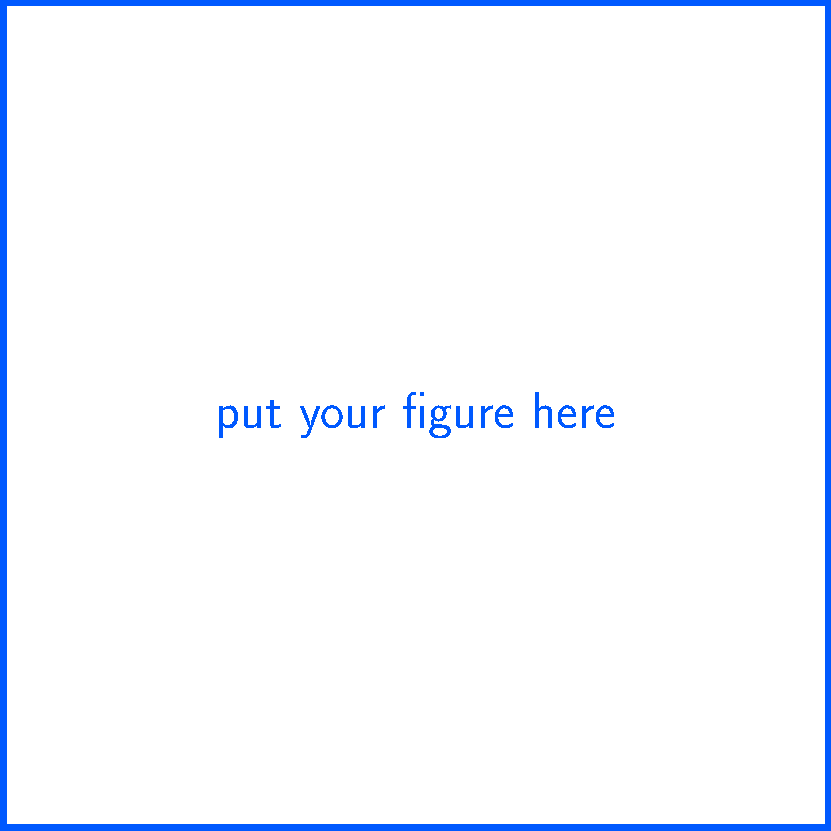
\includegraphics[width=0.24\textwidth]{placeholder.pdf} \hfill
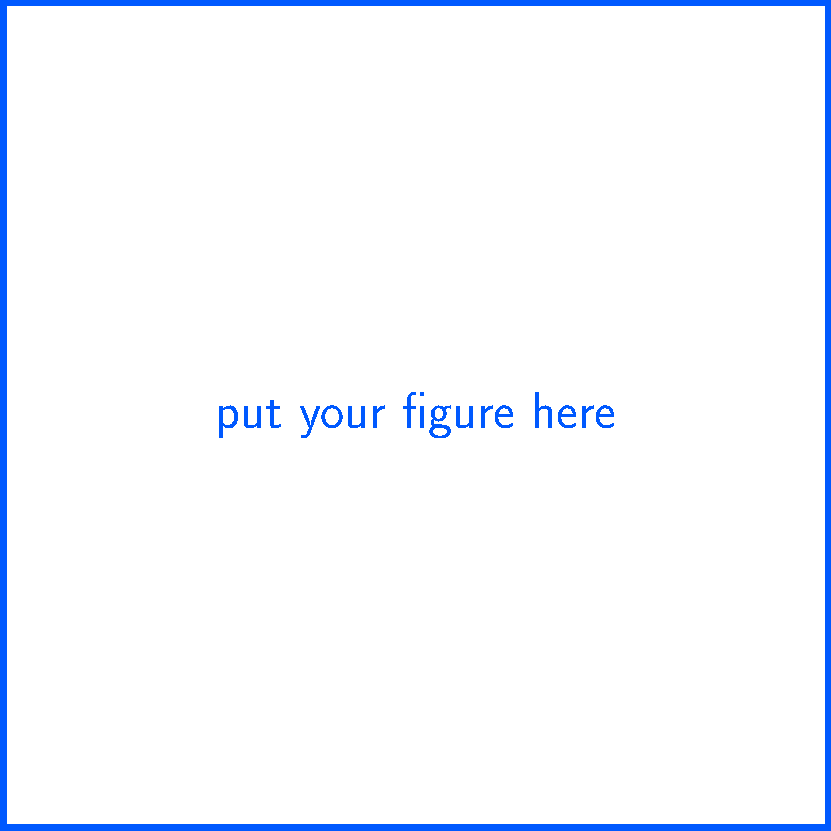
\includegraphics[width=0.24\textwidth]{placeholder.pdf} \hfill
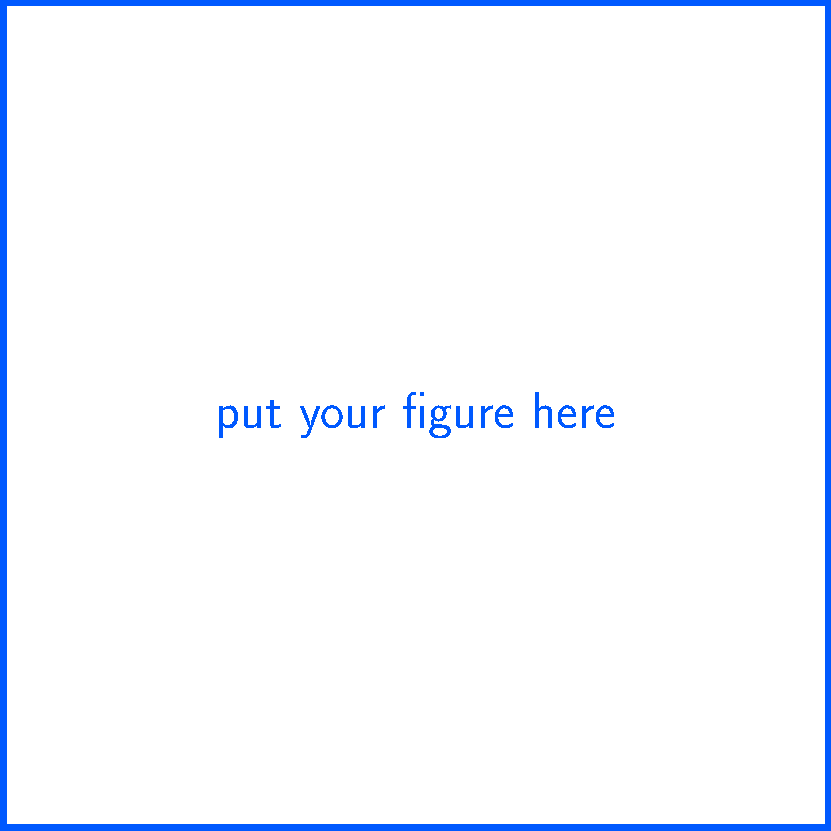
\includegraphics[width=0.24\textwidth]{placeholder.pdf} \hfill
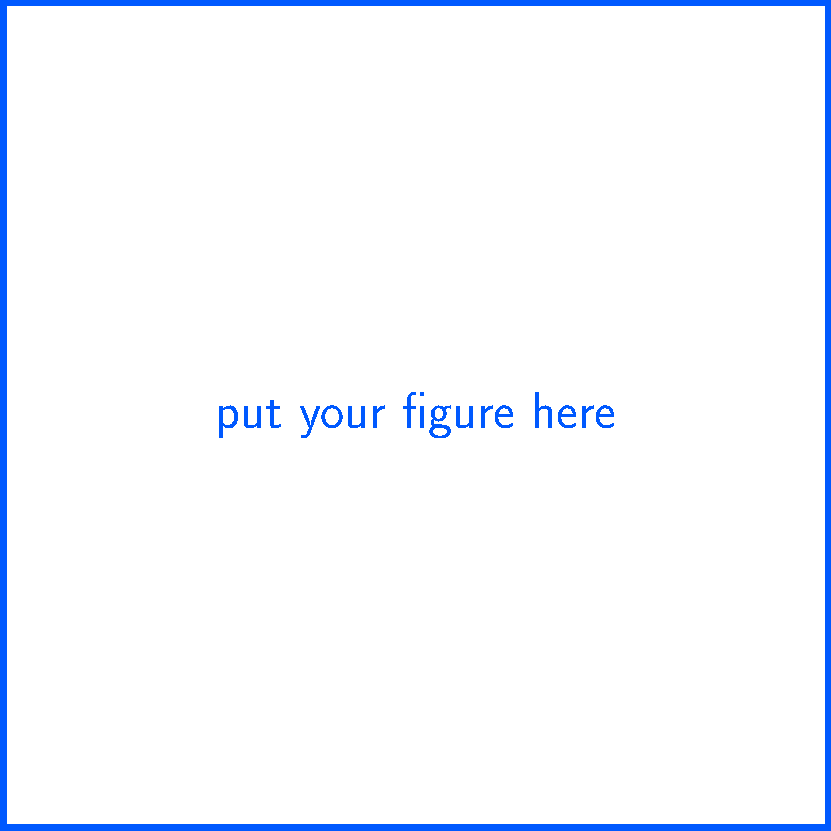
\includegraphics[width=0.24\textwidth]{placeholder.pdf} 
\end{center}
%%%%%
%%%%%
%%%%%
%%%%%
%%%%%



\newpage
Also, paste your code here \\[1ex]
%%%%%
%%%%%
%%%%% enter your code into the following environment
%%%%%
%%%%%
\begin{python}
# paste your code here

\end{python}
%%%%%
%%%%%
%%%%%
%%%%%
%%%%%








\subsection*{task 1.10 \\[1ex] getting used to universal functions}

Again ---without using \keyword{for} loops--- implement a method that turns a given intensity image function $f[x, y]$ into another function $g[x, y]$ where
\begin{equation*}
g \bigl[ x, y \bigr] = \cos \Bigl( f \bigl[ x, y \bigr] \cdot \nu \cdot \tfrac{2\,\pi}{255} \Bigr) \cdot 127.5 + 127.5
\end{equation*}

\vspace{1cm}
Choose $\nu \in \{ 0.5, 1.0, 1.5, 2.0 \}$, apply your method to \texttt{portrait.png}, and enter your resulting images here
%%%%%
%%%%%
%%%%% enter your results here, i.e. replace "placeholder.pdf" by the names of the image files you created
%%%%%
%%%%%
\begin{center}
\includegraphics[width=0.24\textwidth]{t10-0.5.png} \hfill
\includegraphics[width=0.24\textwidth]{t10-1.png} \hfill
\includegraphics[width=0.24\textwidth]{t10-1.5.png} \hfill
\includegraphics[width=0.24\textwidth]{t10-2.png} 
\end{center}
%%%%%
%%%%%
%%%%%
%%%%%
%%%%%



\vspace{2cm}
Also, paste your code here \\[1ex]
%%%%%
%%%%%
%%%%% enter your code into the following environment
%%%%%
%%%%%
\begin{python}
def transform(arrF, nu):
    arrG = np.cos(arrF * nu * 2 * np.pi / 255) * 127.5 + 127.5
    return arrG
\end{python}
%%%%%
%%%%%
%%%%%
%%%%%
%%%%%








\end{document}
